\documentclass[12pt,oneside,a4paper]{article}

\usepackage{./custom}

\usepackage[backend=biber]{biblatex}
\addbibresource{./biblio.bib}

\begin{document}

\begin{titlepage}
\begin{center}

\includegraphics[scale=0.5]{./img/logo_centralesup.jpg} \hfill
\includegraphics[scale=0.3]{./img/logo_digiplante.png}

\vfill 

\textsc{\Large Projet enjeu : Santé et biotechnologies}\\[0.5cm]

\vfill

\textsc{\Large \'Etude documentaire et bibliographique}\\[1.5cm] 

% Title
\HRule \\[0.4cm]
{ \LARGE \bfseries Développement d'outils mathématiques \\ 
   pour l'agriculture de précision \\[0.4cm] }

\HRule \\[1.5cm]

\vfill

{\large
\begin{center}
  \textbf{Groupe SBT-11} \\~\\
\begin{tabular}{rl}
    \quad John &\textsc{de Wasseige} \\
    \quad Nayef &\textsc{Derwiche} \\
    \quad Alexis &\textsc{Mathey} \\
    \quad Daina &\textsc{Zheng} \\ \\
\end{tabular}
\end{center}
}

\vfill

{\large \today}

\end{center}
\end{titlepage}
\newpage

\tableofcontents
\newpage

\section{Résumé}

On résumera ici les enjeux, l'objectif et le livrable du projet défini avec le client
et les principales conclusions de l'étude bibliographique.
\newpage
\section{\'Etude bibliographique}

\subsection{Généralités}
PARLER DES MERISTEMES ?
Tout d'abord, présentons succintement comment se développe et fonctionne une plante. 
Sans doute que la particularité la plus intéressante des plantes, et qui justifie le mieux leur étude est leur capacité à synthétiser de la matière organique (des glucides...) à partir de \ce{CO2}, d'eau et d'énergie solaire. C'est la célèbre photosynthèse qui permet ainsi à la plante de \textit{transformer de la matière minérale en matière organique}, qu'on peut présenter selon cette équation : 
\[
	\ce{6CO2 + 6H2O + \text{énergie solaire} -> C6H12O6 + 02 }
\]
Tous les éléments de la plante participent à ce processus de photosynthèse :
\begin{itemize}
	\item les racines puisent dans le sol l'eau et les sels minéraux nécessaires		
	\item les feuilles captent l'énergie solaire et le dioxyde de carbone (grâce aux cellules chlorophiliennes et aux stomates\footnote{orifice de petite taille situé sur les feuilles qui permet les échanges gazeux entre l'air et la plante})
\end{itemize}

Les sucres ainsi formés apportent l'énergie nécessaire au fonctionnement de la plante et assurent son développement en permettant la synthèse de cellulose qui est l'élément consitutif principal des plantes 
On identifie ainsi les éléments qui agissent sur la croissance de la plante : 
\begin{itemize}
	\item la lumière
	\item l'eau
	\item le dioxyde de carbone
	\item la température : car la température agit sur l'ouverture des stomates et donc sur le flux des échanges gazeux
	\item l'azote, qui permet à la plante de construire les acides aminés nécessaires à l'élaboration des protéines
	\item d'autres minéraux, comme le potassium qui favorise le transfert des assimilat vers les organes de réserve
\end{itemize}
Plusieurs éléments sont donc nécessaires à la croissance de la plante. Parmi eux, on retrouve la lumière, l'eau, le dioxyde de carbone, mais également la température, qui joue un rôle sur louverture ou la fermeture des stomates et régule ainsi les échanges gazeux, lazote, qui permet à la plante de construire les acides aminés nécessaires à lélaboration des protéines, et dautres minéraux comme le potassium, qui favorise notamment le transfert des assimilats vers les organes de réserve il est donc particulièrement important chez la betterave, par exemple ou le phosphore qui joue un rôle dans la photosynthèse.
Chaque feuille 1 participe ainsi à la production de biomasse, qui sera ensuite distribuée à chaque organe en expansion ou nouvellement créé, via lactivité des méristèmes voir section 1.1. Dans la suite, nous regrouperons donc sous le terme de fonctionnement lensemble des mécanismes de production de biomasse par photosynthèse, et dallocation de biomasse aux différents organes de la plante.

\newpage
\section{Contexte du projet}
\subsection{Contexte}
Le problème des ressources \textit{énergétiques} et \textit{alimentaires} est un sujet crucial du  21ème siècle.
Il faudra être capable de nourrir plus de 
9 milliards d'humains en 2050~\cite{wiki:popu_mondiale}.
De plus, les ressources fossiles et l'eau douce viennent à manquer dans certains régions agricoles (comme en Californie). Pourtant, l'agriculture nécessite l'apport d'eau, et est grande consommatrice d'énergie. L'agriculture est ainsi responsable de l'émission de près de 20\% des gaz à effet de serre~\cite{GES}.

\'A l'avenir, il faudra donc optimiser l'agriculture en améliorant les rendements (pour nourrir une population plus grande), tout en réduisant le volume des ressources utilisées (eau et intrants).
D'autre part, le développement de technologies de plus en plus sophistiquées (GPS, drones, etc.) nous permet d'obtenir des données de plus en plus précises.
Cela permet d'envisager le développement d'une agriculture intelligente qui exploiterait ces données grâce à des modèles décisionnels, précis et pratiques et permettrait d'atteindre ce double objectif. On peut ainsi imaginer qu'un jour, un tracteur géolocalisé disperse plus ou moins de graines dans certains zones d'un même champ, afin d'obtenir de meilleurs rendements.

Pour notre part, nous allons nous intéresser à la modélisation de la croissance des plantes et à la pertinence des mesures à réaliser.

\subsection{Présentation du client}
Notre client Pierre Carmier, ainsi que notre référent pédagogique Paul-Henry Cournède sont des chercheurs au laboratoire MAS. 
Ce laboratoire travaille notamment sur les modèles mathématiques de
croissance des plantes, en collaboration avec la startup Digiplante.
Ils ont notamment travaillé sur le modèle LNAS que nous avons décrit
dans notre étude bibliographique.

\subsection{Objectifs poursuivis}
\subsubsection{Implémentation du modèle LNAS sous \textsc{Julia}}
On va travailler sur le Modèle LNAS, adapté à la modélisation du blé. 
Le client a déjà implémenté ce modèle en C++. 
Nous allons pour notre part l'implémenter sous Julia.

Ce modèle était d'abord utilisé pour modéliser la betterave, 
plus simple à modéliser que le blé. 
En effet, pour la betterave il suffit de modéliser 
ses racines (partie utile) et ses feuilles.
On va modéliser le blé, on rajoute la tige et les grains (partie utile du blé)
pour maximiser le rendement des cultures en minimisant l’apport d’intrants.
Nous allons donc utiliser la plateforme Pygmalion pour implémenter ce modèle du blé,
en nous basant sur un document fourni par le client.

Il y a environ 30 paramètres dans le modèle. Une fois le modèle implémenté, nous essaierons donc d'estimer ces paramètres par calibration, grâce aux outils fournis par la statistique.

De plus, les mesures étant difficiles à réaliser et ayant un coût, on ne peut pas mesurer toutes les variables tout le temps. A terme, le but serait \"d'obtenir une méthode permettant d'optimiser le choix des variables à mesurer expérimentalement\", celles qui ont la plus grande influence et dont les mesures sont accessibles. Nous pourrions ainsi réduire l'incertitude sur les prédictions du modèle, en optimisant la calibration.


Le modèle LNAS est un modèle de Markov caché : 
\begin{itemize}
  \item $n$  temps (discret)     
  \item $X_n$ variable au temps $n$       
  \item $Q\sub{grain}, Q\sub{leaf}... $ biomasse des grains, feuilles...      
  \item $f$ fonction qui permet de passer du temps $n$ au temps $n+1$     
  \item $P$ paramètres      
  \item En précipations, température... au temps $n$
\end{itemize}

\begin{equation}
  X_{n+1} = f(X_n,E_n,P,n)
\end{equation} 

$Q\sub{prod}(n)$ proportionnelle à $(1-\exp{(-\lambda \, \text{LAI}(n))})$ 
avec LAI la quantité lumineuse reçue par la plante

C’est un modèle de Markov caché, il n'y a pas de mémoire du passé.
\[
  P(X_{n+1}/X_0,…,X_n) = P(X_{n+1} / X_n) 
\] 

On déduit $Q\sub{grain}(n)$... grâce à $X_n$ et la fonction d'allocation de biomasse.

\newpage
\section{Organisation du groupe}
Nous présenterons dans cette section l'organisation générale du groupe.
On abordera d'abord les outils que nous avons utilisés pour partager 
notre travail le plus efficacement possible.
On présentera ensuite notre manière de gérer la bibliographie
ainsi que les logiciels utilisés pour ne pas perdre les sources visitées.
On détaillera par après l'organisation interne du groupe,
plus précisemment le système mis en place pour optimiser la communication
ainsi que la manière dont les tâches ont été réparties pendant 
ce premier semestre.
On décrira finalement les problèmes, difficultés et risques qui
pourraient survenir, ainsi que nos craintes pour le déroulement du projet. 
Cette dernière partie sera présentée sous
la forme \emph{problème - solution}, afin de décrire les
moyens que nous mettons en \oe{}uvre pour pallier à ces problèmes.

\subsection{Outils de travail collaboratif}
Pour des raisons pratiques et esthétiques, nous avons décider d'écrire
nos rapports en \LaTeX{}.
Il s'agissait donc de trouver la meilleure façon de partager le code source
et de pouvoir contrôler les changements apportés au document.
Une première idée pourrait être d'utiliser ShareLaTeX qui propose une plate-forme
de compilation en ligne ainsi qu'un système de gestion de versions
assez simple à utiliser.
Nous n'avons pas choisi cette solution notamment pour les raisons suivantes.
L'utilisateur doit être connecté dès qu'il veut travailler sur le projet,
le système de compilation est assez lent et l'utilisateur n'est pas libre
d'utiliser son éditeur de texte ou son visualisateur de \textsc{pdf} favori.

Pour palier aux problèmes décrits ci-dessus, le logiciel \texttt{git}
associé à GitHub est une très bonne alternative.
Il permet en effet à chaque membre du groupe de travailler sans être connecté
ainsi que d'utiliser son éditeur et compilateur favori.
Chaque membre travaille donc de son côté en faisant des \emph{commits}
et lorsqu'il juge que son travail est utile pour les autres, 
il \emph{push} sur le serveur.
L'algorithme du fusion, \emph{merge}, permet également de fusionner intelligemment
les lignes d'un fichier qui ont été modifiées par plusieurs membres.
Le dernier point à souligner est que \texttt{git} permet une gestion des branches,
particulièrement pratique lorsqu'on veut développer une partie du projet
sans risquer de créer des erreurs dans le programme principal.

Nous combinons donc ces deux outils pour 
\begin{enumerate}
  \item implémenter le modèle LNAS blé dans la plateforme
  Pygmalion en \textsc{Julia} (une description plus détaillée de
  l'objectif attendu pour cette partie est décrite dans la
  section~\ref{sec:contexte} à la page~\pageref{sec:contexte})
  pour le client dont le code source est sur la plateforme GitLab,
  \item rédiger l'étude documentaire en partageant le code \LaTeX{}
  à l'aide d'un dossier sur 
  GitHub\footnote{\url{https://github.com/jdewasseige/projet-sbt11}}.
\end{enumerate}

\subsection{Gestion de la bibliographie}
Pour la gestion de la bibliographie au sein du document,
nous utilisons le package \texttt{biblatex}.
Celui-ci permet d'écrire l'ensemble de nos références dans un document \texttt{.bib}
sous la forme suivante.
\begin{verbatim}
  @online{histoire_mod_plantes,
    title = {Une histoire de la modélisation des plantes},
    author = {Philippe de Reffye and Marc Jaeger 
    and Paul-Henry Cournède},
    url = {https://interstices.info/jcms/c_38032/une-histoire-de-
    la-modelisation-des-plantes},
    year = {2009},
    month = "04",
  }
\end{verbatim}
La mise en page est alors automatique en fonction des informations fournies
et le rendu de l'exemple est présenté ci dessous.
\begin{figure}[h]
  \includegraphics[scale=0.6]{./img/rendu_elem_bib.jpg}
\end{figure}

Cela parait à priori assez lourd d'écrire soi-même toutes les informations
en suivant cette syntaxe mais il existe des logiciels comme Zotero
qui font le travail à notre place.
Les sources trouvées sur Google Scholar peuvent également être exportées
aisément au format \texttt{BibTex}.

\subsection{Organisation et partage des tâches}
Il nous reste un dernier point à décrire, celui de la \emph{communication}
au sein du groupe.
Nous utilisons Slack\footnote{\url{https://slack.com/}} qui est un logiciel
de plus en plus utilisé pour les travaux de groupe ainsi que dans les start-ups.
Il permet d'éviter de devoir alterner entre plusieurs applications comme les mails,
DropBox et Twitter, puisqu'il permet d'être connecté
à celles-ci au sein de l'application.
On peut également créer plusieurs \emph{channels} pour séparer la communication
entre les différentes tâches.
Par exemple dans ce projet nous avons les \emph{channels} suivantes :
\texttt{general}, \texttt{etude-documentaire}, 
\texttt{planning} et \texttt{dev\_plate-forme}.
On trouve aussi un système d'historique et de gestion de fichiers efficace.

L'ensemble des tâches ainsi que leur répartition pendant l'année
est associé au planning \textsc{Gantt} qui se trouve
dans l'Annexe~\ref{ann:planning} à la page~\pageref{ann:planning}.

\subsection{Risques, difficultés et problèmes potentiels}
Nous avons identifié plusieurs risques, difficultés et problèmes qui pourrait survenir durant le projet et ralentir sa mise en oeuvre: 

\begin{itemize}
	\item Une perte partielle ou totale de nos données, à cause d'une mauvaise manipulation sur les plateformes de travail, dont le contenu peut être modifié/supprimé par chaque utilisateur.
	\item Nous n'arrivons pas à acquérir les compétences informatiques nécessaires pour implémenter et travailler sur les modèles informatiques de modélisation de plantes.
	\item Un seul élève du groupe réalise la plupart du travail (parce qu'il est le seul à savoir coder par exemple). Cela conduirait à une perte de communication et de motivation au sein du groupe.
	\item Peu de communication avec notre client, et en conséquence mauvaise compréhension du projet et de ses objectifs. 
\end{itemize}

Pour éviter que cela n'arrive, nous allons :
\begin{itemize}
	\item utiliser la plateforme GitHub qui permet de récupérer les sauvegardes précédentes.
	\item nous partager équitablement les tâches
	\item faire en sorte que chaque membre du groupe comprenne chacune des étapes de notre travail.
	\item échanger et essayer de rencontrer régulièrement notre client, profitant de sa proximité, étant chercheur au laboratoire MAS de Centrale.
\end{itemize}
\newpage
\section*{Conclusion}
\addcontentsline{toc}{section}{Conclusion}

Les perspectives qu'offre l'étude de la croissance des plantes sont des plus stimulantes.
En effet, les enjeux sont cruciaux. Les plantes sont un élément clé de notre économie. A la base de nos régimes alimentaires, elles sont également source d'oxygène, d'énergie avec l'émergence des agro-carburants, et sont utilisées dans la construction, l'industrie des vêtements et même dans l'industrie pharmaceutique.

Dans le même temps, pour répondre à une demande de plus en plus forte, l'agriculture a recours à l'irrigation intensive, aux engrais et aux pesticides pour augmenter ses rendements. Malheureusement, ces méthodes ont un impact négatif sur l'environnement et leur utilisation n'est pas viable, comme en témoigne par exemple le quasi-asséchement de la mer d'Aral à cause d'une culture intenisive du coton~\cite{aral}.
 
Heureusement, la science, aidées des mathématiques et d'une collecte de données devenue omniprésente, semble plus que jamais capable de développer une agriculture viable et productive. Pour cela, elle bénéficie de plusieurs siècles d'études des plantes qui ont permis d'affiner leurs connaissances.



\newpage
\section*{Remerciements}
\addcontentsline{toc}{section}{Remerciements}

Nous tenons à remercier notre client Pierre Carmier, pour son temps précieux et sa pédagogie. 
Nous remercions également Mme Le Chevallier et Mme Lopes, qui guident les étapes de notre projet, pour leurs remarques et leurs retours sur nos présentations et l'avancement de notre projet.
Merci également aux encadrants des Activités de Développement Personnel et Leadership, qui nous aident à cohésionner le groupe et à mieux nous connaître.
\newpage

%\documentclass{ctexart}
\usepackage{tikz}
\usetikzlibrary{trees}
\tikzset{box/.style={rectangle ,rounded corners=5pt, draw}}
\begin{document}
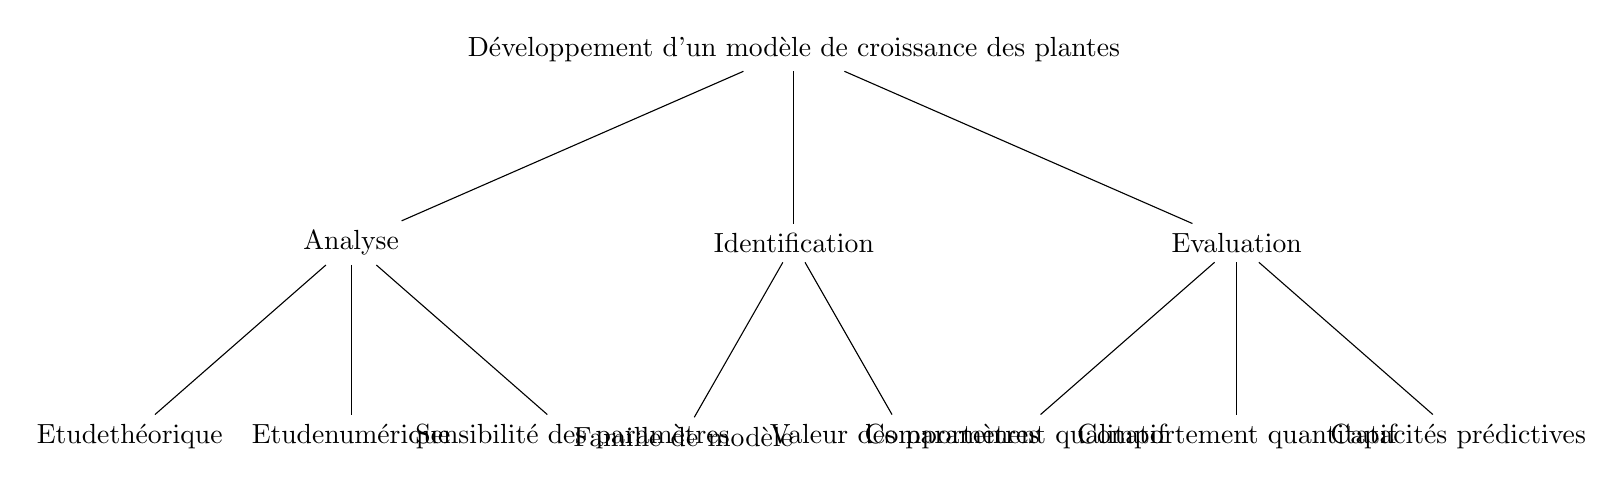
\begin{tikzpicture}[level distance=70pt, sibling distance=5pt]
  
\tikzstyle{level 1}=[sibling distance=160pt]
\tikzstyle{level 2}=[sibling distance=80pt]
\tikzstyle{level 3}=[sibling distance=200pt]
%\tikzstyle{level 4}=[sibling distance=50pt]
%\tikzstyle{level 5}=[sibling distance=80pt]
%\tikzstyle{level 6}=[sibling distance=50pt]
%\tikzstyle{level 7}=[sibling distance=80pt]
%\tikzstyle{level 8}=[sibling distance=50pt]
%\tikzstyle{level 9}=[sibling distance=80pt]

\node{Développement d’un modèle de croissance des plantes}
  child { node {Analyse}
    child { node {{Etude\\ théorique}} }
    child { node {Etude \\ numérique}}
    child { node {Sensibilité des paramètres}}
    }
    child { node {Identification}
    child { node {{Famille de modèle}} }
    child { node {Valeur des paramètres}}
    }
    child { node {Evaluation}
    child { node {{Comportement qualitatif} }}
    child { node {Comportement quantitatif}}
    child { node {Capacités prédictives}}
    };
\end{tikzpicture} 
\end{document}
%\newpage

\addcontentsline{toc}{section}{Bibliographie}
\nocite{*}
\printbibliography
\newpage

\appendix
\part*{Annexes}
\section{Planning}
\label{ann:planning}

\begin{figure}
  \begin{center}
    \includepdf[scale=0.8]{./annexes/planning_gant.pdf}
  \end{center}
\end{figure}\newpage
\section{Fiche objectif}
\label{ann:fiche_obj}
\begin{figure}[H]
  \begin{center}
  \includegraphics[scale=0.61,angle=90]{./annexes/fiche_objectif.pdf}
  \end{center}
  \caption{Fiche objectif représentant une analyse globale du projet.}
  \label{fig:fiche_obj}
\end{figure}
\subsection{Arbre de pertinence}
\begin{figure}[h]
  \includegraphics[scale=0.51]{./annexes/arbre_de_pertinence.pdf}
  \caption{arbre_de_pertinence \textsc{Gantt} de répartition le projet en petites tâches.}
  \label{fig:arbre_de_pertinence}
\end{figure}

\end{document}